\documentclass{article}
\usepackage[english]{babel}
\usepackage{babel} % voor nederlandse afbreekregels e.d.
\usepackage{hyperref} % voor links, hier niet gebruikt
\usepackage{graphicx} % voor importeren van figures, hier niet gebruikt
\usepackage{tabularx} % voor tabellen met controle over kolombreedte, hier niet gebruikt
\usepackage{booktabs} % voor nettere tabellen dan de standaard
\usepackage{enumerate} % voor controle over nummering van items
\usepackage{amssymb,amsmath,amsthm,amsfonts} % van de AMS, voor nettere math
\usepackage{qtree} % voor het maken van mooie bomen, hier niet gebruikt
\usepackage{mathabx} %voor het \notdivides commando, niet gebruikt
\usepackage{adjustbox}
\usepackage{listings}
\usepackage{color}
\usepackage{pifont}
\usepackage{algorithm} % pseudocode
\usepackage[noend]{algpseudocode} %pseudocode 
\usepackage{sectsty}

%\DeclareGraphicsExtensions{.pdf,.png,.jpg}

\title{Research Report BEP}

\renewcommand{\baselinestretch}{0.9} 

\sectionfont{\fontsize{11}{15}\selectfont}

\renewcommand{\qedsymbol}{\hfill \emph{QED}}

% document variables:
\newcommand{\cMysename}{Research Report}
\newcommand{\doctitle}{Elvan Kula \& Hans Schouten}
% ---

\newcommand{\cmark}{\ding{51}}%
\newcommand{\xmark}{\ding{55}}%

\newcommand{\itab}[1]{\hspace{0em}\rlap{#1}}
\newcommand{\tab}[1]{\hspace{.2\textwidth}\rlap{#1}}

% http://tex.stackexchange.com/questions/110328/formatting-a-logical-pd-derivation:
\newcommand{\fgh}[1]{\fvline%
  \makebox[0pt][l]{{%
      \raisebox{-1.4ex}[0pt][0pt]{\rule{#1}{\arrayrulewidth}}}}%
  \hspace*{\fitchindent}}
  
  \lstset{language=Java,
%alles tussen "//(*" en "*)" wordt als TeX code verIrkt
	escapeinside={//(*}{*)}} 
 


\newcommand*\xor{\mathbin{\oplus}}
% Fill these in:

% if you use algorithms, this is a nice one:
% http://www.lirmm.fr/~fiorio/AlgorithmSty/
%\usepackage[algo2e]{algorithm2e}

\makeatletter

\makeatother

%%%%%%%%%%%%%%%%%%%%%%%%%%%%%%%%%%%%%%%%%%%%%%%%%%%%%%%%%%%%%%%%%%%%%%%%%%%%%%%%
%% document start
%%%%%%%%%%%%%%%%%%%%%%%%%%%%%%%%%%%%%%%%%%%%%%%%%%%%%%%%%%%%%%%%%%%%%%%%%%%%%%%%
\begin{document}
\thispagestyle{empty}

\begin{center}

\vspace*{2cm}
{\huge \cMysename}

\begin{center}
    \line(1,0){450}
\end{center}

{\LARGE \doctitle}

\vspace{1cm}


\end{center}
\newpage

\tableofcontents
\newpage
%%%%%%%%%%%%%%%%%%%%%%%%%%%%%%%%%%%%%%%%%%%%%%%%%%%%%%%%%%%%%%%%%%%%%%%%%%%%%%%%
%% end of front page
%%%%%%%%%%%%%%%%%%%%%%%%%%%%%%%%%%%%%%%%%%%%%%%%%%%%%%%%%%%%%%%%%%%%%%%%%%%%%%%%

\section{Introduction}

\paragraph{Target Customers}
Aircraft and airport noise are complex subject matters which have been studied for decades and are still the focus of many research efforts nowadays. Also at the department of Air Transport \& Operations (ATO) at TU Delft’s Faculty of Aerospace Engineering. ATO has three research aims: 1) To develop radical new ways to optimize aircraft operations for efficiency, safety, cost and environmental impact; 2) To extend the analysis to an airline fleet and network level to include capacity and resilience; 3) To synthesize these to include operational safety at an airline and ATM level. To support their research findings at conferences, the researchers at ATO need a standalone application for model-based optimization and visualization of aircraft noise. This report summarizes the research phase of this project, during which we familiarize ourselves with the field and investigate what programming language, libraries, tools, etc. are best suited for our product.

\paragraph{Customer Needs}
We will provide a product that represents a creative and efficient way to minimize and visualize aircraft noise along simulated and real flight routes. This requires the implementation of two mathematical models: one for the computation of noise contours and one for the iterative optimization of aircraft trajectories for minimum noise and population annoyance. The models will be deployed by the research team to predict aircraft noise along a particular trajectory (flight route) and to update the trajectory design in an iterated manner to minimize the produced noise over populated areas around airports. Therefore, the parameters that take part in the optimization of aircraft trajectories range from the generic criterion of contour areas to a number of site-specific criteria based on the impact on population

Additionally, the program should be able to visualize the noise produced along the trajectory through a 3D animation pictured on a real map. This requires a visualization of noise contours, which are ‘noise footprints’ whose shape indicate areas of constant noise. Noise contours are a new subject to the research group and have not been implemented in relation with noise minimization before so this will be a challenging topic for us. The visualization should also show the effects of the produced aircraft noise on population annoyance.

In this orientation report we summarize the results of the research phase of this project as follows: first in Section 2 we give some more detailed information on the applications that we will extend and on similar products in the field. Section 3 focuses on the requirements gathering for this project, including a description of the various interviews we have conducted as well as the main requirements we identify. Section 4 then describes our chosen approach based on these requirements, including what programming language and tools we will use. Finally, Section 5 details what quality guarantees we will provide and how these are verified.
\section{Background}
 
The functionality addressed by our client requires the implementation of four models: noise model, noise contouring model, trajectory optimization model and the visualization model. For our project, we have investigated the documents with background information on these models that were provided by the client.

In the first section we will further describe the way these models work and the way our product will incorporate them. We also compare the functionality of our product with existing work. The Noise Model and Noise Contouring Model are further detailed in Sections 2.1.1 and 2.1.2 respectively. Then we will describe the original approach to the trajectory optimization and compare this with the new approach suggested by the ATO department in Section 2.1.3. The second Section covers existing software on related work. We will look into software provided by the client and visualization in Google Earth with KML objects.

\subsection{Documentation on Calculation Models}

\subsubsection{Noise Model}

The general algorithm of noise calculation is based on empirically obtained noise-power-distance (NPD) tables. The first step consists of interpolating for the current thrust level and slant range (observer ↔ aircraft) to find the uncorrected noise metric. Since the NPD-tables are created under the assumption that the aircraft flies on an infinitely long segment at a given reference speed a number of corrections need to be applied. For more information on the methodology you are referred to the INM7.0b Technical Manual.

\subsubsection{Noise Contouring Model}

The methodology for calculating the contour areas partly follows the standard closest point search common in contouring algorithms, but differs in the fact that It will avoid incorrectly forming multiple contours when in reality only one single closed contour exists. In the case that contour areas are required the spline representation is used to refine the grid to cells of 125x125 m. After refining the grid, all the switch points in the new grid are located. Switch points are points on the axes of the grid cells in which the noise value changes from a value higher than to a value lower than the requested contour value. After gathering all switch points within the grid, the points need to be ordered to form a continuous string. For this purpose, starting in point $i$, candidate points for $i+1$ are located and evaluated for feasibility. This process is further explained in detail in documentation about the NoiseLAss tool v2.0. 

\subsubsection{Trajectory Optimization for Minimum Noise}

In general, an optimization of the noise impact requires criteria that range from the generic criterion of contour areas to a number of site-specific criteria based on the impact on population or on enforcement points. Enforcement points are locations in the vicinity of the airport at which a maximum value for a specific noise metric is defined. This value is then used for regulatory purposes to control the noise exposure near the airport. 

The optimization algorithm first gathers the noise input on an arbitrary grid with cell size gx and gy, where gx is not necessarily equal to gy, allowing for a grid consisting of non-square cells. The original grid is then used to define a set of b-spline coefficients, which form the basis for a b-spline interpolation of the data. For all site-specific criteria the spline coefficients are directly used to find the noise values in the requested observer or enforcement points by evaluating the b-spline in the required coordinates.

\subsection{Related Work}
Software tools that implement the four models already exist and are already being used in the aerospace industry and research field. The problem is that these tools lack automation and function as separate executables. Currently there is no program that executes all these models in a pipelined manner. In this section we will only discuss the tools that are currently used by the ATO department since our program will incorporate algorithms equal or similar to the ones used in these tools.

\subsubsection{INMTM v3.0} The Noise Model is implemented in this noise calculation tool created by respectively the TU Delft and the NLR. It implements the FAA’s standard methodology for noise assessments. Since 1978 this has been the standard Integrated Noise Model (INM) in over 65 countries. The tool computes noise levels expressed in six time-based metrics at a user-specified regular grid based upon finite flight-segment data. It requires two user-provided text files: one describing the full trajectory expressed in a number of nodes and one defining a 2-dimensional (no elevation data) or 3-dimensional grid for noise calculation.

The calculations in this tool are conform world standards and are performed below one second. The client was content with this tool and therefore we decided to re-use and (if needed) further improve the tool in our final program. 

\subsubsection{NoiseLAss v2.0} The noise contouring algorithm and optimization model are implemented in this noise level assessment tool. The tool is basically a collection of assessment criteria which can be retrieved according to user specification whilst using a common input and output format. 

The NoiseLAss tool calculates the noise levels in the enforcement points by interpolating the user-supplied noise input data on the specific point. This allows the user to define other points at which the noise level is of interest. 

Additionally, the tool contains a number of dose-response relationships to assess the direct impact on population for six different noise metrics. These relationships can be used to quantify the impact of commercial aviation on near-airport communities for daytime and night operations, e.g. the number of expected awakenings due to a single night-time flyover and due to cumulative noise metrics. 

Although the model is directly compatible with the output files of the INMTM v3 noise calculation tool, it still requires user supplied input files and does not perform real-time. Therefore the client wants us to build the contouring and optimization models from scratch for our program following the algorithms used in this tool.

\subsubsection{Visualization with Google Earth KML Objects}
KML (Keyhole Markup Language) is a file format used to display geographic data in an Earth browser such as Google Earth. KML uses a tag-based structure with nested elements and attributes and is based on the XML standard. KML also enables the user to store tours and animations in Google Earth. Since KML meets all the requirements of our flight animation and since the ATO department is already familiar with this file format, KML seemed a perfect fit for our project. Next to KML we also considered alternatives like CityGML and Geography Markup Languages. Although these alternatives are fine, KML is better integrated with Google Earth. Therefore we decided to use KML objects with the Google Earth API for visualization in our program. 

\section{Requirements}
For the process of requirements gathering we have mainly focused on interviewing our client Dr. Ir. Sander Hartjes, who is also a representative of the ATO department because of his academic function. He is equipped to inform us how the research department applies the mathematical models and what features in our program they would benefit from most. The resulting requirements and the main results of the interviews will be described in this section as follows: we summarize the results of these interviews in Section 3.1 and give a list of the requirements in Section 3.2. 

\subsection{Interviews}

To get a clear view of the customer's needs we interviewed our client Dr. Ir. Sander Hartjes during two extensive meetings of two hours each. Besides this, other meetings were also held with him to discuss and clarify the aerospace engineering part of the project. This was necessary since we did not have any knowledge of the theories of noise contouring and noise minimization before the project. 

Dr. Ir. Sander Hartjes is employed as an Assistant Professor in the field of airline operations at the chair of Air Transport and Operations. His research mainly focuses on optimal aircraft performance regarding the reduction of noise and pollutant emissions. He has already been working at ATO since 2008 and therefore he is equipped to inform us on the way the department is going to use our program and what features the department will benefit from most.

Through our first interview with Sander we learned that the ATO department lacks a visualization tool for its research findings at conferences. The researchers, including Sander, still manually transform Matlab files containing trajectory coordinates into KML files and enter this into Google Earth for visualization. Sander told us that they increasingly need this process to be automated when dealing with large trajectories. This would spare a lot of their time that goes into manually importing flight data from Matlab into KML. Sander also informed us that their preference goes out to visualization in Google Earth since this is commonly used in their research field.

Additionally, the current visualization only consists of a simple animation of an airplane following a particular path in Google Earth. Sander told us that they would like to be able to visualize noise contours in a real-time 3D animation. The ATO researchers create noise contour diagrams with 3D model simulation software such as AutoCAD, but currently there is no way for the department to animate noise contours that are produced along a particular trajectory. Sander let us know that the implementation and visualization of noise contours in Google Earth is a crucial requirement for the program.

During our second interview Sander informed us, after consultation with other researchers of the department, that they would like our program to visualize noise contours not only in relation with produced noise levels but also regarding to iterative optimization of flight trajectories for minimum noise. Therefore, an optimization algorithm needs to be implemented that should not only take the actual measured noise volumes into account but also the area of the noise contours. The trajectories would then be optimized based on the volume and spreading of the noise. Recent studies show that the timing and spreading of noise affect the population annoyance greatly and thus they are potentially important factors in the minimization of noise. This way of minimizing aircraft noise and visualizing noise contours is not only new to the ATO department but also to the research field itself. Noise contours are normally used to regulate sound and not as an indication for the optimization of trajectories.

Finally, when Sander showed us the tools that are currently used by the ATO department to calculate noise values and optimize trajectories, we noticed that these tools also lack automation. At the moment ATO researchers manually transform the output of the noise model in the right data form and then enter it into the optimization model. The research department would benefit greatly by an automated and pipelined execution of these processes in a standalone application. 

\subsection{Requirements}
Below we present an initial list of formal requirements for the program. Additionally, we provide an extended list of user stories to specify the required behavior of the program in different scenarios.

\begin{itemize}
\item The program can calculate noise values in real time.
\item The program can calculate and output the actual noise contours that are produced along a particular trajectory in real time.
\item The program has the option to optimize a trajectory in an iterated manner to minimize the produced noise over populated areas that are affected. The optimization algorithm should be based on the area of the produced noise contours instead of the actual noise values.
\item The program can visualize the (optimal) trajectory together with the noise contours in real-time 3D animation mapped on Google Earth.
\item The program can calculate and visualize the effects of produced noise on population annoyance using the awakenings algorithm.
\item The program should save the results of the visualization and, if requested, the intermediate calculated values in a particular format and directory specified by the user.
\item The program should execute all the processes above (corresponding to the computation of noise values, noise contours, noise minimization and the visualization of noise contours) in an automated and pipelined manner.
\item The program should offer all these tasks in a graphical user interface.
\end{itemize}

\subsection{User stories and scenarios}
The main requirements that a user of the system will actually notice are most clearly presented in so-called user stories. These stories describe what the results of an action will be for a certain user. Unfortunately, some of the other requirements or design decisions can not be represented in the same format that easily, since they do not really involve a user in the classic sense of the word. Instead some of the functions that the program should be able to use have been described in scenario format.

The user stories that describe the behavior as presented to the user can be summarized as follows:

\subsubsection{Must have features} 
These features are must haves since the program would not be functioning and meet the (minimal) requirements of the customer without these implemented. 

\noindent\rule{8cm}{0.4pt} \\
\begin{itemize}
\item \textbf{Given} I am an ATO Researcher and I want to specify a grid and trajectory,
\item \textbf{When} I read in an arbitrary data file (.dat extension) or text file indicating the input flight trajectory and grid (based on the RD-coordinate system),
\item \textbf{Then} the program should be able to handle this input without any problems.
\end{itemize}
\noindent\rule{8cm}{0.4pt}\\
\begin{itemize}
\item \textbf{Given} I am an ATO Researcher and I want to save the resulting visualization,
\item \textbf{When} I click the button to save the 3D animation,
\item \textbf{Then} the program should save the used data and settings in the specified directory.
\end{itemize}
\noindent\rule{8cm}{0.4pt}\\
\begin{itemize}
\item \textbf{Given} I am an ATO Researcher and I want to easily access a saved visualization during a conference, 
\item \textbf{When} I select the file representing the previously stored visualization,
\item \textbf{Then} the program should automatically start the visualization without requiring any further user interaction.
\end{itemize}
\noindent\rule{8cm}{0.4pt} \\
\begin{itemize}
\item \textbf{Given} I am an ATO Researcher and I want to calculate noise levels produced along a particular trajectory,
\item \textbf{When} I click the button to start the noise calculation,
\item \textbf{Then} the program should calculate and output four types of noise levels; A-Weighted Sound Exposure Level (SEL), Effective Perceived Noise Level (EPNL), A-Weighted Maximum Sound Level (LAMAX) and Tone-Corrected Maximum Perceived Noise Level (PNLTM).
\end{itemize}
\noindent\rule{8cm}{0.4pt} \\
\begin{itemize}
\item \textbf{Given} I am an ATO Researcher and I want to calculate noise contours produced along a particular trajectory,
\item \textbf{When} I have selected the decibel value(s) I am interested in and the program has finished calculating the noise levels (former step),
\item \textbf{Then} the program should automatically start calculating the noise contours along the given trajectory for the decibel values I have selected.
\end{itemize}
\noindent\rule{8cm}{0.4pt} \\
\begin{itemize}
\item \textbf{Given} I am an ATO Researcher and I want to save the calculated noise contours,
\item \textbf{When} I click the button to save the noise contour,
\item \textbf{Then} the program should save the noise contour as a csv file in the specified directory.
\end{itemize}
\noindent\rule{8cm}{0.4pt} \\
\begin{itemize}
\item \textbf{Given} I am an ATO Researcher and I want to optimize a particular trajectory by minimizing the noise produced by the aircraft,
\item \textbf{When} I select the option to optimize the trajectory,
\item \textbf{Then} the program should start and keep updating the trajectory until no optimization is possible.
\end{itemize}
\noindent\rule{8cm}{0.4pt} \\
\begin{itemize}
\item \textbf{Given} I am an ATO Researcher and I want to visualize a particular trajectory and the produced noise contours,
\item \textbf{When} I select the option to visualize the trajectory,
\item \textbf{Then} the program should show a real-time 3D animation mapped on Google Earth in a separate window.\\
\end{itemize}
\noindent\rule{8cm}{0.4pt} \\

\subsubsection{Should have features}
These features are should haves since the basic components of the program would work without these features but it would be better (meet the requirements of the customer better) if these would be implemented. 

\noindent\rule{8cm}{0.4pt}\\
\begin{itemize}
\item \textbf{Given} I am an ATO Researcher and I want to easily access a saved visualization during a conference, 
\item \textbf{When} In windows explorer I double click the file representing the previously stored visualization,
\item \textbf{Then} Windows should automatically launch our application and start the visualization without requiring any further user interaction.
\end{itemize}
\noindent\rule{8cm}{0.4pt}\\
\begin{itemize}
\item \textbf{Given} I am an ATO Researcher and I chose the wrong input file,
\item \textbf{When} I notice my mistake during the program run and I want to disrupt or cancel the current operation,
\item \textbf{Then} the program should abort the current operation after I clicked the cancel button.
\end{itemize}
\noindent\rule{8cm}{0.4pt}\\
\begin{itemize}
\item \textbf{Given} I am an ATO Researcher and I want to analyze a real flight route from the FlightRadar24,
\item \textbf{When} I select to use FlightRadar24 as data source and specify a flight,
\item \textbf{Then} the program should fetch all data of the selected flight and start the noise calculation and visualization.
\end{itemize}
\noindent\rule{8cm}{0.4pt}\\

\subsubsection{Could have features} 
These features are could haves since they are not necessary to the customer and to the functioning of the program but it would be nice to include them if there is enough time left in our timeframe. 

\noindent\rule{8cm}{0.4pt}\\
\begin{itemize}
\item \textbf{Given} I am an ATO Researcher and I want to analyze an active flight from the FlightRadar24,
\item \textbf{When} I select to use FlightRadar24 as data source and specify a flight,
\item \textbf{Then} the program should start fetching the data of the selected flight and start the noise calculation and visualization in real time.
\end{itemize}
\noindent\rule{8cm}{0.4pt}\\
\begin{itemize}
\item \textbf{Given} I am an ATO Researcher and I want to make an adjustment to a particular data element in the input file,
\item \textbf{When} I import the file and double click a particular data element,
\item \textbf{Then} the program should enable me to adjust the clicked data element.
\end{itemize}
\noindent\rule{8cm}{0.4pt}\\
\begin{itemize}
\item \textbf{Given} I am an ATO Researcher and I want to specify a grid and trajectory,
\item \textbf{When} I read in a Matlab file (.mat extension) indicating the input flight trajectory and grid (based on the RD-coordinate system),
\item \textbf{Then} the program should be able to handle this input without any problems.
\end{itemize}
\noindent\rule{8cm}{0.4pt}\\
\begin{itemize}
\item \textbf{Given} I am an ATO Researcher and I want to estimate how long I have to wait for the results of the program, 
\item \textbf{When} I clicked the button to start the noise calculation,
\item \textbf{Then} the program should continuously show me the current progress with a progress bar.
\end{itemize}
\noindent\rule{8cm}{0.4pt}\\
\begin{itemize}
\item \textbf{Given} I am an ATO Researcher and I want to share the program with others,
\item \textbf{When} I start the program.
\item \textbf{Then} the program should be recognizable in a blink by showing its name and logo.
\end{itemize}
\noindent\rule{8cm}{0.4pt}\\

\subsubsection{Won't have features} 
These features are won't haves since the customer does not actually need these features to be implemented. There probably won't be enough time left for the following features but it could be interesting for a follow-up phase of the project. 

\noindent\rule{8cm}{0.4pt}\\
\begin{itemize}
\item \textbf{Given} I am an ATO Researcher and I want to log all my activities in the program,
\item \textbf{When} I click the logger button,
\item \textbf{Then} the program should create a text file with an overview of the input files I entered and visualized during the current program run.
\end{itemize}
\noindent\rule{8cm}{0.4pt}\\
\begin{itemize}
\item \textbf{Given} I am an ATO Researcher and I want to make a memo of my own reflections on the input or output data,
\item \textbf{When} I double click a data element in a file,
\item \textbf{Then} the program should enable me to add a comment to the clicked data element.
\end{itemize}

\subsubsection{Scenarios}
Whereas some scenarios will be developed as new features are picked to be implemented, a few scenarios that result in the automated execution of the program are given here:

\noindent\rule{8cm}{0.4pt} \\
\begin{itemize}
\item \textbf{Given} an input file indicating the trajectory and grid,
\item \textbf{When} the user selects to optimize and start the noise calculation,
\item \textbf{Then} the program should perform all operations including visualization in an automated manner without the user needing to perform any additional actions.\\
\end{itemize}
\noindent\rule{8cm}{0.4pt} \\
\begin{itemize}
\item \textbf{Given} a particular trajectory and its corresponding noise contours (calculated by the program),
\item \textbf{When} the user has selected the option to optimize the trajectory,
\item \textbf{Then} the program should optimize the trajectory based on the area of the noise contours instead of the actual noise values.
\end{itemize}
\noindent\rule{8cm}{0.4pt} \\


\section{Approach}
In this section we will describe our approach to the project, starting with the development methodology as described in Section 4.1. In Section 4.2 we present a broad overview of our system design. The programming languages and tools we will use for the project are specified in Sections 4.3 and 4.4 respectively. Finally, the API of FlightRadar24 will be introduced in Section 4.5.

\subsection{Development Methodology}
During the software development phase, the team will be applying agile development methods. In particular, the Scrum development framework will be used. Alternatives we have considered include the waterfall methodology and XP, extreme programming.

We have opted not to use the waterfall method due to its rigid and inflexible nature. For this project we foresee having to cope with design changes, which is difficult and time-consuming once implementation has started in the waterfall method. Throughout the project we will be implementing multiple mathematical models and designing a GUI that should be responsive and user-friendly in all situaions. In practice, the design of a GUI often has to go through multiple revisions to accomodate new requirements, incorporate new insights in the problem, etc. 

On the other hand, agile methods feature an iterative approach to software development, and are flexible enough to alter the design of a product throughout a project. As a result, using an agile method enables us to focus on the core of the product during initial stages, and add more functionality as the project progresses. It also allows us to keep a list of features that are not required for a functional product, but would increase its usefulness if implemented. These features can be reprioritized based on the client’s demands to ensure the final product contains the most requested and most valuable features that could be implemented in the limited timeframe.

Our choice for Scrum over XP as the preferred agile method is mainly based on experience of the team working with Scrum. On top of this, extreme programming is less suitable for small teams due to its strict requirements on code reviewing and testing, i.e., using pair programming. Due to the limited time available for this project, in some situations we prefer being able to work in parallel to ensure we cover more features. 
Additionally, in Scrum the work to be performed is planned in the sprint planning. We will work with one-week sprints. At the beginning of every week we will describe our goals for that week in a sprint plan. At the end of the week, all the items on the sprint plan need to be finished, fully tested and committed to the repository. A sprint reflection should also be made in which we discuss our progress during that sprint and possible improvements for the next sprint. Section 5 contains more detail on how we will ensure sufficient quality using our chosen methodology.

\subsection{System Overview}

\begin{figure}[ht]
    \centering
    \label{img:architecure}
    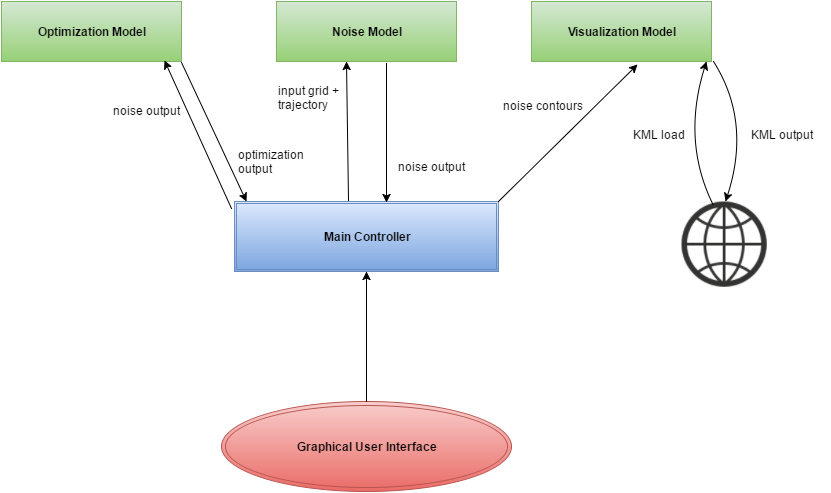
\includegraphics[width=0.75\textwidth]{images/EmergentArchitecture}
    \caption{A broad overview of the system architecture}
\end{figure}

As depicted in the diagram above, the models present the subsystems of our program. The Noise Model is responsible for the calculation of the noise values produced along a particular trajectory. Based on these noise values the Contour Model computes the noise contours that the user is interested in. Then
the Optimization Model updates a trajectory in an iterated manner based on the calculated noise contours. The KML Writer creates the KML files based on the (optimal) trajectory and its noise contours. These KML files will automatically be entered into Google Earth for visualization. Changes to the KML files will automatically be transferred to Google Earth by a 'KML load' script, which periodically loads the files into Google Earth.

The subsystems exchange their outputs with the main presenter which uses the output of one subsystem as input for the next one. This happens according to the following pipeline:

\begin{enumerate}
\item The main presenter enters the initial input file of the user into the Noise Model.
\item The main presenter passes on the output of the Noise Model to the Contour Model.
\item If the user selected the option to optimize, the main presenter relegates the output of the Contour Model to the Optimization Model. Otherwise, the output of the Contour Model is directly passed on to the KML Writer. When the output of the Contour Model is first handed over to the Optimization Model a loop is initiated: the current trajectory is updated by the Optimization Model and the workflow of the program starts all over again by entering the updated trajectory as input into the Noise Model. This optimization process is repeated until no further optimization is possible. 
\item The main presenter relegates the output of the Contour Model and the coordinates of the (optimal) trajectory to the KML Writer.
\end{enumerate}

Following this method the models are executed in a pipelined manner. But the subsystems will be designed in such a way that, given the right input files, the subsystems can also be run separately from each other and function as standalone applications.

\subsection{Programming Languages \& Libraries}

Because our program needs to solve optimization problems that require running computationally expensive calculations on a large amount of data points, code performance is an important factor. To this end, we hesitated between C++ and C\# and decided to compare them. 

C++ is known to be able to support high performance applications. However, we stumbled upon a few articles and blogs in which the performance of C++ was compared to C\#. All these articles noted that C++ itself does not have speed advantages. It is the fact that highly experienced programmers can express the strengths of the  language correctly which makes C++ code in some cases favorable over C\#. From these statements one can conclude that a performance-conscious C\# programmer can write programs with a performance similar to a well-written C++ program, however with the ease of being programmed in C\#. Since we both are not that experienced with C++, being able to write high quality C++ code and to actually achieve a higher performance would take practice and time to learn and thus would be very time consuming for us. This could even negatively affect the functionality of our program. Therefore, we believe that the use of C\# over C++ will increase our productivity. Even if a programmer succeeds to get a better performing implementation, the performance increase of C++ would probably not weigh up to the additional features that could have been added as a result of the time saved by programming in a more straightforward language. 

Besides that, C++ has cross platform capabilities whereas C\# depends upon the .NET framework which restricts its use to only the Windows platform. However, the benefit of having cross platform capabilities is not that important in our case since the client will use the software in combination with Matlab and Google Earth in a Windows environment. Therefore, we considered a few of the required components of our program with C++ and C\# in our minds. Our program needs to be able to generate XML files, PNG files and will make use of a library with a collection of common data structures. After a quick search on Internet we noticed that such libraries were more easy to find for C\#. Also, C\# is specifically designed to work with the .Net framework and is geared to the modern environment of Windows and user interface. Therefore C\# offers a lot more functionality and flexibility for GUI programming. With C++ you would have to hand code a lot of GUI functionality.

Mainly the first consideration regarding code performance and the GUI functionality that is built in C\# seemed to us as valid reasons for choosing C++ over C\#. To this end, we choose C\# as the main language for our code.

\paragraph{.NET Framework for GUI Development}
After we decided to choose C\# as the main language for our code, it was an obvious choice to develop our GUI with the .NET framework. The .NET Framework has become the mainstream environment for new Windows applications. It offers a lot of fancy options in case we decide to use innovative UI objects. Besides, the .NET framework contains a lot of predefined libraries for graph rendering and the creation of PNG's and color maps (which we are actually going to need for the visualization model). This helps to eliminate the amount of unnecessary codes and involves less coding for the developers. The framework also supports System.XML, which lets applications work with XML-defined data, including using XSLT and XPath. This comes in handy for us since we are going to use KML objects that are based on XML-defined data for the visualization model of our program.

But we still had to decide between using Windows Forms or WPF. The single most important difference between WinForms and WPF is the fact that while WinForms is simply a layer on top of the standard Windows controls (e.g. a TextBox), whereas WPF is built from scratch and doesn't rely on just the standard Windows controls. This might seem like a subtle difference, but it really isn't, which you will definitely notice if you are either creating a very complex or a relatively easy GUI. Since WinForms restricts users to a collection standard windows controls, a GUI that requires control elements that deviate from this is almost impossible to construct. By default WinForms for example does not support adding a background image to a ListView component. A programmer who really wants to seek the limits of what is graphically feasible will stumble upon a vast number of restrictions in WinForms. With WPF on the other hand control elements can be created by the designer in a container like fashion. In WPF for example a button with background image is created by adding a panel containing the image to the button. This is a great strength of WPF, however the current WPF form designer makes designing forms in WPF more tedious since you have to do significantly more work yourself. To give an example, the alignment of control elements requires more effort and is less obvious in WPF compared to WinForms. Since our GUI will mainly focus on requesting parameters that are required for performing the calculations, no complex control elements nor heavy graphics are necessary. Therefore, for our Windows application in which the standard Windows look and feel is expected WinForms will suffice and with the currently superior design environment will save us precious time.

\subsection{Tools usage}
In order to develop a product of this size, both development and process tools can help to keep an overview of the tasks at hand. In order to easily keep track of the increasing number of lines of code, a good IDE and some version control software can be very insightful. Similarly planning tools such as the agile-orientated JIRA can help to provide a clear overview of the current ToDo-list. In Section 4.5.1 we describe the development tools we will use in this project, whereas Section 4.5.2 will focus on the process tools.

\subsubsection{Functionality Tools}
\paragraph{INMTM v3.0} This noise calculation tool was provided by our client. It implements the FAA’s standard methodology for noise assessments and therefore the calculations in this tool are conform world standards. The client is really content with this tool since its execution time is less than one second. Therefore we decided to re-use the tool in our final program. In our minds we hold the option for further performance improvements in later stages of our project. The tool is written in Fortran so this means that, if we would like to improve the performance further, we would need to learn Fortran in a short period of time or we would need to rewrite the entire noise model from scratch. This is something we should take in consideration depending on the overall performance of our end product and the customer's needs.

\paragraph{Google Earth} Our client informed us that their preference goes out to visualization in Google Earth since this is commonly used in their research field. Besides, Google Earth provides a lot of options for satellite imagery of the entire earth in an interactive format. Compared to all its alternatives like Marble and Here Maps, Google Earth provides the most complete satellite imagery of the entire earth in 3D. One disadvantage of Google Earth is that the resolution of the image varies depending upon the location. This may make it more difficult for the user to view certain areas that are isolated or uninhabited. But since our visualization will mainly be located in the Netherlands and in populated areas surrounding airports, this should not be a problem for our program.

\subsubsection{Development tools}
As has been previously described in Section 4.4, we will develop the largest part of our code in C\#. For this part of the code, we will use Visual Studio. Visual Studio is both commonly used for C languages and is an IDE we have experience with. The alternative in the form of SharpDevelop has been considered, but since we have experience with Visual Studio, we believe this will allow for a smoother workflow and switching to the similar but slightly different SharpDevelop would hold no advantages. In contrast to an extensive IDE such as Eclipse, the alternative of Vim has also been considered. Vim is a command-line text editor that offers many development features for those that are used to its somewhat peculiar set of shortcuts. The downside is that for large projects it is quite difficult to keep a clear overview of all code. 

In addition to an IDE, we will also require version control to easily keep track of code changes. Version control systems manage changes in code and/or documents, and provide a central location to store the code and documents. We choose Git as our version control tool. Our project team has experience with both Git and SVN, and both version control systems are commonly used in academia and industry. As we are using an agile development method, a working version of the product, preferably with new features, should be presentable at the end of every sprint. To maintain a stable version of the product, branched development can be a huge benefit. This allows for a main branch that contains the proven to be stable version of the software, with new features being developed in separate branches. Because Git has built-in support for branch-based development, it is preferred over SVN which offers a very primitive branching system which involves manually creating the folders for branches and merging them afterwards.

Given that the core of our application is written in C\#, multiple testing frameworks are available. Out of the different options we decided to go with NUnit, since it is the most similar one to JUnit  which the team has the most experience with. Additionally, NUnit integrates seamlessly with Visual Studio and it fully supports test class inheritance. MsTest has slightly more features for test logging, but we still choose for NUnit due to it’s native support in Visual Studio and our previous positive experience with JUnit.

\subsubsection{Process tools}

In addition to the tools required for the development, we are also using a planning tool to keep track of our planning. JIRA is an online tool that allows for an overview of the current work, as well as some scrum-oriented features. One of these features is the scrum board which mimics the structure of ToDo, Work in Progress, Done that is often done with sticky notes on a white board. 

\subsection{API}

\paragraph{FlightRadar24 for real-time flight data}
For visualization of real flight routes we are going to use the API of FlightRadar24 to gather real-time air flight data. Its current version provides the broadest coverage of aggregated flight tracks and abstract information. The data is retrieved by a network of ADS-B receivers. FlightRadar24 does not provide a public API but they have a streaming endpoint for their data in JSON. We will be using a PHP API which is developed by a third party and provides all these data in JSON.

We considered the alternative API of FlightAware. They seem to have better routes/ flight plan data than FlightRadar24 but their feed is 5 minutes delayed. Because we want to visualize real flight routes (near) real-time, the delayed feed is no option for us. Another potential alternative is the OpenSky Network. This is a free open-source API that provides live visualization of air traffic and a real-time flight data feed. In contrast to FlightRadar24 it also offers access to historical raw data which would be very useful for testing our program. However, the location data feed is not that accurate and it contains no information on the flight status, such as the type of plane.

\section{Quality Guarantees}
In this section we talk about the quality of both the process and the code. In Section 5.1 we talk about the type of documentation we use in the code and why. In Section 5.2 we talk about the way we write and run tests. In Section 5.3 we will discuss the evaluation of the quality of our code, and how we guarantee the quality of our reports and documents.

\subsection{Documentation}
Two different types of documents will be required for this project, the first being documentation of the process, including this document, the second being code documentation. All documents related to the process will be produced in LaTeX, supplemented with BibTeX when references are a part of the report. For these documents the version control system Git will also be used.

For our project, we choose to use the built in documentation tags in Visual Studio and Doxygen for documentation. The reason for using Doxygen is that it is one of the most popular documentation generation tools available for C\# and numerous other programming languages like C and Python and therefore requires a flexible documentation generation tool. We choose either the standard deployed by Visual Studio or Doxygen if there is no standard, to generate documentation for the extensions.
\subsection{Testing}
As new functionalities are added to a product, it is always important to verify that existing functionality is not broken during the latest update. To this end a test suite containing both unit tests an integration tests can be a great help. To evaluate our code, we use test-driven development. With test-driven development,

Unit-tests are written before the code that should be tested. This allows us to specify the working of our code through the tests that is initially based on our design choices. These tests often take the form of user stories: ”I am X and if I do Y, then Z will happen”. The use of a test-driven development approach leads to spending less time on debugging code, and to more modular and extensible code in general. Additionally, we want our code to be well-thought-out and ensure that both team members have a large understanding of the code. To this end, the unit-tests for a certain part of the product code are written by a different team member than the actual product code.

Simply writing the tests is of course not sufficient for them to be useful, since tests also need to be run to get any data out of it. A continuous integration server with hooks into Git allows you to have the tests run automatically on every push to the server. We will use this hook to run our unit tests using mocks after every push. Jenkins is a commonly used example of such a continuous integration platform and is also the one we will be using for this project. Though we have some experience with CruiseControl as well, Jenkins is more commonly used and provides all the required features. Testing in a live environment will be done at the end of every sprint, outside of the continuous integration tools.

\subsection{Evaluation}
Because we want to deliver a high-quality product to our customer, we evaluate both our code and documents carefully before delivery. To this end, we use multiple methods.

All documents we deliver are written using an iterative method. This means all sections are both read and edited by the other team member. This method has the following benefits:
\begin{itemize}
\item Both team members are aware of document contents.

\item Section contents are refined and reflect the accurate opinion of the team.
\end{itemize}

At the end of the development process, we use benchmarking techniques to evaluate the performance of our software. Because the ATO department is going to use the program for actual flight trajectories, obtaining real-world representative workloads is a non-trivial task. The performance evaluation will consist of running real flight routes as input.

\end{document}
%%%%%%%%%%%%%%%%%%%%%%%%%%%%%%%%%%%%%%%%%%%%%%%%%%%%%%%%%%%%%%%%%%%%%%%%%%%%%%%%